\documentclass[10pt]{article}
\usepackage[margin=0.82in]{geometry}
\usepackage{booktabs,tabularx,array}
\usepackage[table]{xcolor}
\usepackage{graphicx}
\usepackage{microtype}
\usepackage{enumitem}
\usepackage[hidelinks]{hyperref}
\graphicspath{{figures/}}
\definecolor{InkBlue}{HTML}{17324D}
\definecolor{PaleBlue}{HTML}{E8F2FB}
\definecolor{PaleGray}{HTML}{F3F6F9}
\newcommand{\Hit}{\textsc{Hit@1}}
\title{Execution Mode as Context for Behavior-Based Attack Activity Association}
\author{}
\date{Open research draft · 30 October 2026}

\begin{document}
\maketitle
\section{Motivation and research question}

AI agents are changing how cyber operations are carried out. AttackAgentDetect brings execution mode into attack-behavior analysis as a new evidence dimension and develops reproducible methods to study how human, scripted, and Agent execution reshapes trace association and AI-era threat characterization.

Behavioral association is an established computational task: HOLMES correlates suspicious information flows in host-audit traces to produce campaign evidence; OSTINATO compares behavior and TTPs across hosts; POIROT and ActMiner align CTI-derived attack graphs with provenance graphs; HERCULE, ATLAS, and FALCON reconstruct multi-stage attack stories from correlated logs \cite{holmes,ostinato,poirot,actminer,hercule,atlas,falcon}. These methods use command or event sequences, TTPs, entity relations, and causal structure as evidence. Their evaluation targets differ, but each demonstrates a concrete role for behavioral association in investigation. Practitioner frameworks likewise track activity clusters before assigning named actors \cite{unit42}.

Execution mode is already part of documented cyber operations. Anthropic's 2025 report describes human operators coordinating Claude Code agents and MCP tools across a multi-stage campaign; MITRE records the activity as Campaign C0062 \cite{anthropic,mitrec0062}. Alongside association systems that connect audit behavior, operation sequences, and causal relations, these reports establish execution mode as a timely behavioral dimension for investigation and threat profiling. AIT/AECID provides adjacent log-based Human/LLM classification for IT troubleshooting \cite{ait}. We extend this line of work by evaluating how log-derived mode scores change activity association.

\section{Data and protocol}

We use the pinned CC BY 4.0 release of Cyber Task Horizons (revision \texttt{178c0da1800f9\allowbreak c07311e1b8d\allowbreak 6c61dd8104e7b\allowbreak 4e7b4ae}) \cite{cth}. It contains task-based CTF evaluations and expert terminal recordings. We select InterCode-CTF, CyBench, and NYU CTF Bench, the three suites with overlapping human and Agent task records. The resulting corpus has 177 non-empty traces in 40 benchmark-qualified task groups: 57 expert terminal records and 120 Agent tool-call records. InterCode-CTF contributes 27 groups (40 human, 81 Agent), CyBench 6 (8 human, 18 Agent), and NYU CTF Bench 7 (9 human, 21 Agent).

\begin{table}[t]
\centering
\caption{Trace sources in the evaluated intersection.}
\label{tab:data}
\small
\rowcolors{2}{PaleGray}{white}
\begin{tabularx}{0.84\linewidth}{>{\raggedright\arraybackslash}Xrrr}
\toprule
\rowcolor{InkBlue}\textcolor{white}{Benchmark} & \textcolor{white}{Task groups} & \textcolor{white}{Human} & \textcolor{white}{Agent} \\
\midrule
InterCode-CTF & 27 & 40 & 81 \\
CyBench & 6 & 8 & 18 \\
NYU CTF Bench & 7 & 9 & 21 \\
\rowcolor{PaleBlue}\textbf{Total} & \textbf{40} & \textbf{57} & \textbf{120} \\
\bottomrule
\end{tabularx}
\end{table}

Human records are terminal-input transcripts; Agent records are structured bash tool calls. For both, we extract allowlisted command names and coarse action categories. Prompts, task descriptions, outputs, model names, timestamps, and paths are excluded; 300 Python calls are omitted from primary features. The release instructs human experts not to use AI, but remote collection cannot independently verify this. The labels therefore describe released trace sources, not independently adjudicated decision-maker identity.

The primary protocol uses three benchmark-stratified outer folds grouped by benchmark/task, with seed \texttt{20261030}. Every query is ranked against all other held-out traces from the same benchmark and fold, with no mode filtering; the mean gallery contains 29.325 candidates. The evaluation label records whether two traces solve the same benchmark-qualified challenge. It is not a shared intrusion, activity, campaign, or actor label. Five additional seeds estimate split sensitivity. Task groups are the unit of metric aggregation and bootstrap resampling. We report task-macro \Hit, mean reciprocal rank (MRR), Recall@5, and nDCG@5. Intervals use 5,000 paired benchmark-stratified task-cluster bootstrap draws conditional on fitted folds.

The behavior ranker combines command cosine, ordered action-bigram cosine, ProcGrep BPE/Jensen--Shannon similarity, and command-length similarity. A task-supervised ranker learns from same-task versus different-task pairs. The mode-aware ranker adds execution-mode scores generated out of fold within each training partition. Pair labels depend only on task identity; test labels and source metadata are excluded from inference. ProcGrep is a pinned third-party adaptation, not a method introduced by this project.

\section{Results}

\subsection{Initial mixed-gallery retrieval protocol}

The mixed gallery gives a random-ranking \Hit{} of 0.189. Command cosine reaches 0.600; ProcGrep reaches 0.594; the task-supervised behavior ranker reaches 0.571. Mode-aware ranking is highest on the fixed primary split at 0.607, a +0.036 paired change over the task-supervised ranker (95\% CI [+0.006, +0.069]). Against command cosine, the change is +0.008 (95\% CI [−0.046, +0.059]). Across the five alternate splits, the mode-aware minus task-supervised change averages −0.007 (95\% CI [−0.026, +0.012]). The positive primary-split estimate therefore does not persist across the split-sensitivity check.

\begin{table}[t]
\centering
\caption{Mixed-gallery task retrieval on the primary split. Higher is better.}
\label{tab:retrieval}
\small
\rowcolors{2}{PaleGray}{white}
\begin{tabularx}{\linewidth}{>{\raggedright\arraybackslash}Xrrrr}
\toprule
\rowcolor{InkBlue}\textcolor{white}{Method} & \textcolor{white}{\Hit} & \textcolor{white}{MRR} & \textcolor{white}{Recall@5} & \textcolor{white}{nDCG@5} \\
\midrule
Command TF--IDF cosine & 0.600 & 0.695 & 0.648 & 0.618 \\
Action bigram cosine & 0.565 & 0.657 & 0.591 & 0.567 \\
ProcGrep BPE/JSD & 0.594 & 0.676 & 0.551 & 0.544 \\
Length only & 0.514 & 0.636 & 0.543 & 0.514 \\
Task-supervised behavior & 0.571 & 0.669 & 0.600 & 0.576 \\
\rowcolor{PaleBlue}\textbf{Mode-aware behavior} & \textbf{0.607} & \textbf{0.693} & \textbf{0.619} & \textbf{0.604} \\
Mode only & 0.281 & 0.483 & 0.433 & 0.366 \\
\bottomrule
\end{tabularx}
\end{table}

\begin{figure}[t]
\centering
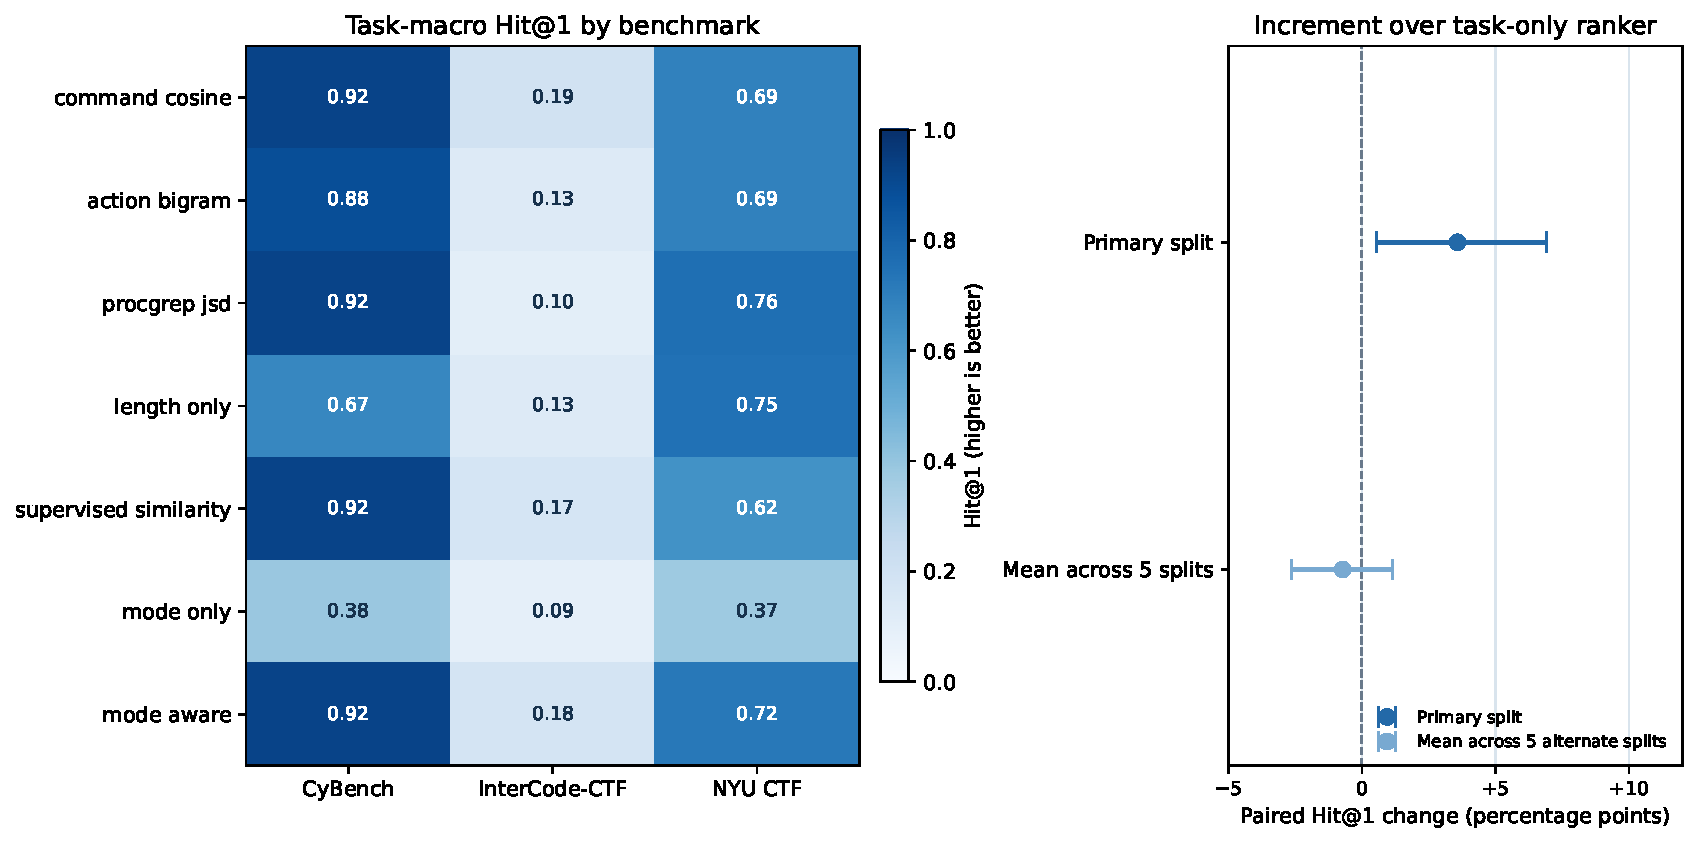
\includegraphics[width=\linewidth]{mixed_gallery_retrieval.pdf}
\caption{Benchmark-level task retrieval and paired mode-score changes. The right panel shows the primary estimate and the average across five alternate task splits; the dashed line marks no change.}
\label{fig:retrieval}
\end{figure}

At a 0.5 threshold on Platt-calibrated held-out scores, the mode classifier's pooled confusion matrix is $[[43,14],[8,112]]$ for Human/Agent rows, corresponding to record-level balanced accuracy 0.844. Fold scores are 0.912, 0.883, and 0.738. Platt calibration is fit on training-task out-of-fold predictions and reduces test Brier score from 0.110 to 0.089. These measurements show that the two released record types are separable in this corpus. Because label and capture interface coincide, they do not establish recognition of an unknown operator.

\begin{figure}[t]
\centering
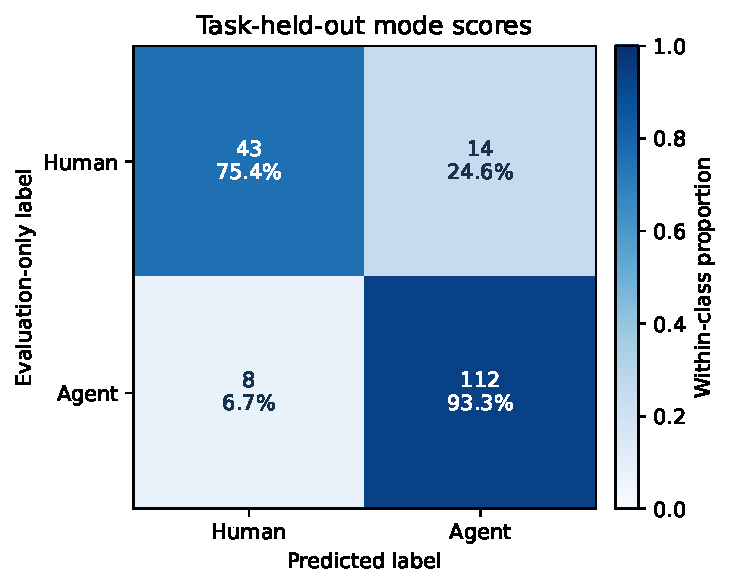
\includegraphics[width=0.63\linewidth]{mixed_gallery_confusion.pdf}
\caption{Task-held-out Human/Agent trace-label confusion matrix. Cells show counts and within-class proportions.}
\label{fig:confusion}
\end{figure}

\subsection{Association errors at a training-only threshold}

Retrieval metrics do not show the errors made when the system decides whether to connect a pair. We therefore evaluate pairwise decisions under a nested protocol: each outer training fold supplies three inner task-held-out folds for threshold selection; the outer test tasks remain untouched. Each method receives its own threshold, selected to maximize task-macro balanced accuracy on inner out-of-fold pairs. A test pair is linked when its score meets that threshold. We compare command cosine, the task-supervised behavior ranker, its mode-aware extension, and a command-length control. The target is same-task matching within the released CTF benchmarks, not real attack-activity matching.

The mode-aware ranker reaches task-macro balanced accuracy 0.669 (95\% task-cluster CI [0.611, 0.722]), compared with 0.612 [0.568, 0.657] for the behavior-only ranker. The paired increase is 5.7 percentage points [3.4, 8.1]. Against command cosine, however, the increase is 0.6 points [−4.1, 4.8], leaving no clear gain over this simpler baseline.

The pair-type breakdown shows where the mode score changes decisions. Relative to behavior-only ranking, it lowers the false-split rate for same-task H--Agent pairs from 0.317 to 0.191 (−12.6 points, 95\% CI [−17.7, −7.6]) while raising the false-merge rate for different-task H--Agent pairs from 0.387 to 0.472 (+8.4 points, [3.4, 13.2]). Execution-mode context therefore reduces one cross-mode matching error while increasing another; the result supports conditional use of this signal, not a universal correction.

\begin{table}[t]
\centering
\caption{Task-held-out pairwise association errors. Each method's decision threshold is selected on inner training-task out-of-fold pairs. Entries are task-macro rates with 95\% task-cluster bootstrap intervals. Relevance labels denote the same CTF challenge.}
\label{tab:association-errors}
\small
\rowcolors{2}{PaleGray}{white}
\begin{tabularx}{\linewidth}{>{\raggedright\arraybackslash}Xrrr}
\toprule
\rowcolor{InkBlue}\textcolor{white}{Method} & \textcolor{white}{False split} & \textcolor{white}{False merge} & \textcolor{white}{Balanced accuracy} \\
\midrule
Command cosine & 0.377 [0.288, 0.470] & 0.296 [0.198, 0.399] & 0.664 [0.597, 0.731] \\
Task-supervised behavior & 0.275 [0.185, 0.371] & 0.501 [0.433, 0.569] & 0.612 [0.568, 0.657] \\
\rowcolor{PaleBlue}\textbf{Mode-aware behavior} & \textbf{0.238 [0.148, 0.343]} & \textbf{0.423 [0.363, 0.491]} & \textbf{0.669 [0.611, 0.722]} \\
Length-only control & 0.195 [0.122, 0.277] & 0.600 [0.506, 0.689] & 0.602 [0.531, 0.677] \\
\bottomrule
\end{tabularx}
\end{table}

\begin{figure}[t]
\centering
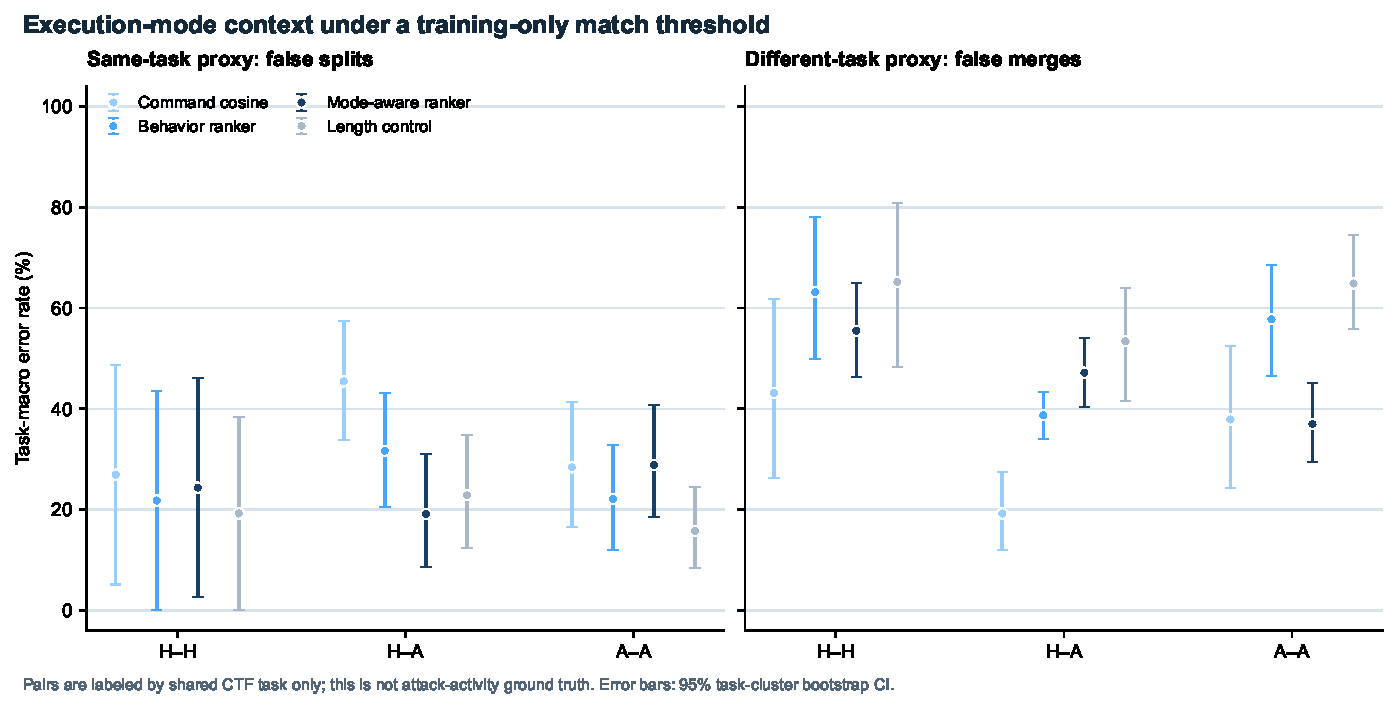
\includegraphics[width=\linewidth]{association_error_rates.pdf}
\caption{False-split and false-merge rates stratified by pair mode. H--A denotes a pair of records labeled Human and Agent in the dataset. The same-task H--H estimate uses 17 task groups; all other strata use 40. Error bars are 95\% task-cluster bootstrap intervals.}
\label{fig:association-errors}
\end{figure}

\subsection{Feature signal and fixed-operating-point association}

We test whether execution-mode labels can be separated from three observable input groups: trace size and coarse action mix, command vocabulary, and operation-sequence statistics. F0--F2 are single-group baselines. F1 is command-name TF--IDF over unigrams and bigrams; F2 contains nine fixed statistics: adjacent-command and adjacent-action repetition, action-switch rate, unique-command ratio, normalized mean and maximum action-run lengths, command/action bigram repetition, and a short-trace flag. F3 concatenates F1 with F2. This ablation supports the broader question of whether execution mode can inform behavior-based activity association. F3 versus F1 isolates the added value of sequence statistics given command vocabulary. On task-held-out traces, command TF--IDF reaches balanced accuracy (BA) 0.849 with logistic regression and 0.866 with ExtraTrees. Fixed sequence statistics alone reach 0.648 and 0.642. Adding these statistics changes BA by $-2.0$ points for logistic regression (95\% task-cluster CI [$-8.3$, $+3.3$]) and $+1.4$ points for ExtraTrees ([$+0.3$, $+2.5$]); their contribution is classifier-dependent.

\begin{table}[t]
\centering
\caption{Task-held-out execution-mode source-label classification. Values are task-macro BA with 95\% task-cluster intervals.}
\label{tab:feature-ablation}
\small
\rowcolors{2}{PaleGray}{white}
\begin{tabularx}{\linewidth}{>{\raggedright\arraybackslash}Xccc>{\centering\arraybackslash}p{1.55cm}>{\centering\arraybackslash}p{1.55cm}}
\toprule
\rowcolor{InkBlue}\textcolor{white}{Feature set} & \textcolor{white}{Count + action mix} & \textcolor{white}{Command TF--IDF} & \textcolor{white}{Sequence statistics} & \textcolor{white}{Logistic BA} & \textcolor{white}{ExtraTrees BA} \\
\midrule
F0: Coarse baseline & $\bullet$ & -- & -- & 0.643 & 0.635 \\
F1: Command vocabulary & -- & $\bullet$ & -- & 0.849 & 0.866 \\
F2: Sequence structure & -- & -- & $\bullet$ & 0.648 & 0.642 \\
\rowcolor{PaleBlue}\textbf{F3: Command TF--IDF + operation-sequence statistics} & -- & $\bullet$ & $\bullet$ & \textbf{0.828} & \textbf{0.880} \\
\bottomrule
\end{tabularx}
\smallskip
\footnotesize $\bullet$ included; -- excluded. BA is task-macro balanced accuracy (higher is better). The primary ablation, F3 $-$ F1, is $-2.0$ percentage points for Logistic Regression (95\% CI [$-8.3$, $+3.3$]) and $+1.4$ points for ExtraTrees ([$+0.3$, $+2.5$]).
\end{table}

On the matched cohort with at least four commands (99 traces, 25 tasks), full command sequences outperform their first-four-command prefixes by 8.8 points for TF--IDF (95\% CI [+2.0, +15.7]); shuffling command order yields a +3.1-point change whose interval crosses zero. These results locate most measured separability in command content and observation amount, not a stable order signature.

\begin{figure}[t]
\centering
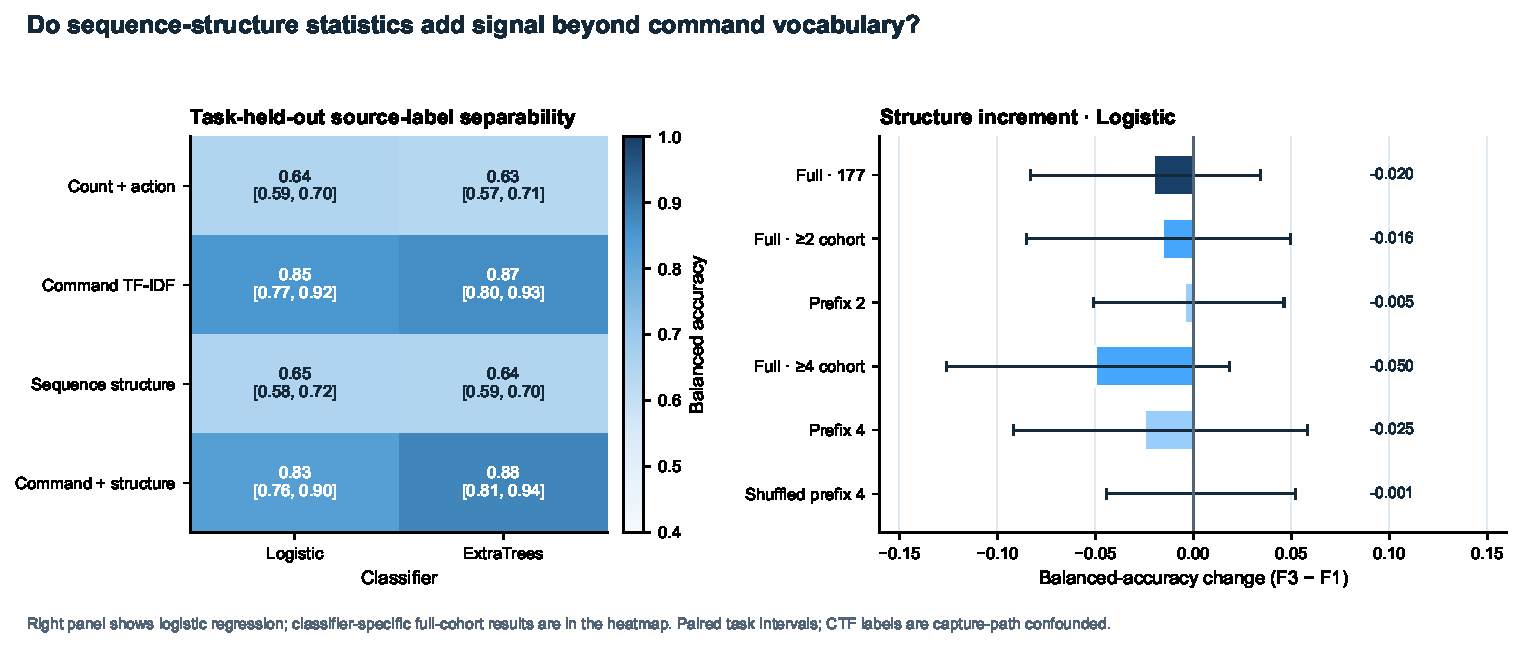
\includegraphics[width=\linewidth]{feature_ablation_v1.pdf}
\caption{Source-label separability and paired feature increments. The right panel shows the logistic-regression increment across matched cohorts; the left panel reports both classifiers. Labels remain confounded with capture interface.}
\label{fig:feature-ablation}
\end{figure}

\begin{figure}[t]
\centering
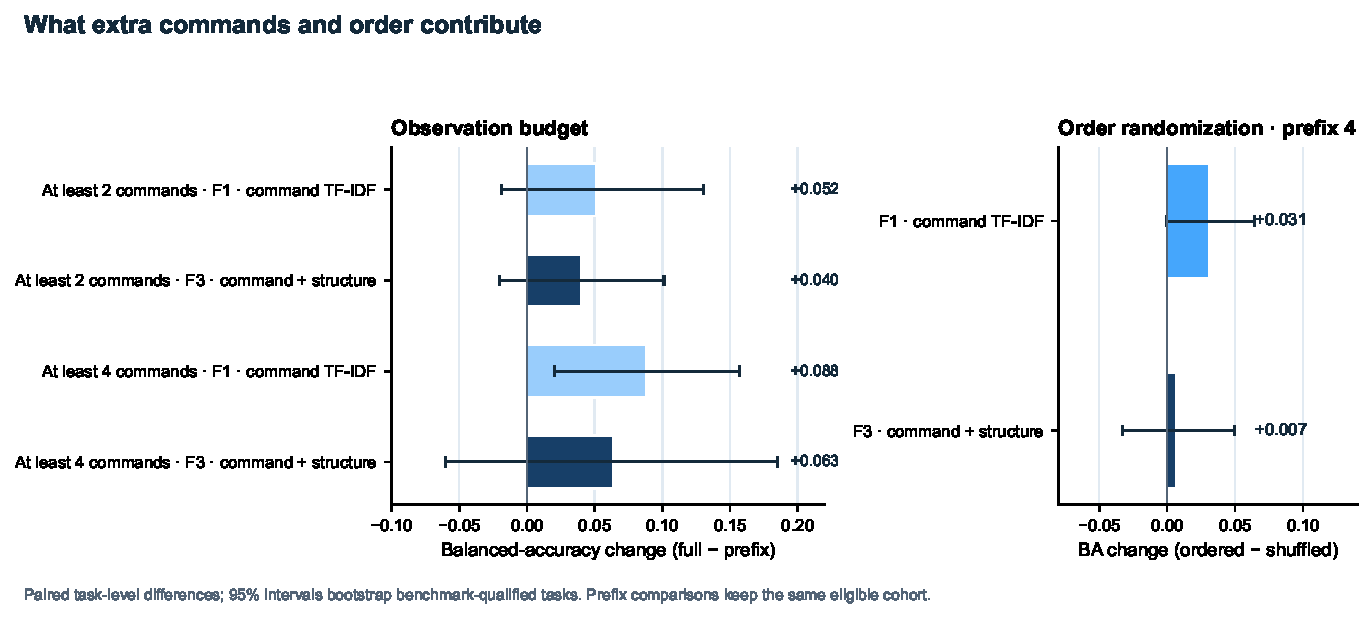
\includegraphics[width=\linewidth]{feature_budget_order_v1.pdf}
\caption{Matched-cohort changes from observing full traces instead of prefixes and from preserving versus shuffling command order.}
\label{fig:feature-budget-order}
\end{figure}

For association, thresholds are selected within each outer training fold to keep task-macro false merges at or below 20\%, then minimize false splits. At this operating point, mode-aware ranking attains Hit@1 0.607 versus 0.571 for the behavior ranker (paired change +3.6 points, 95\% CI [+0.6, +6.8]). Same-task Human--Agent false splits fall by 12.7 points ([$-19.0$, $-6.5$]), while different-task Human--Agent false merges rise by 11.9 points ([$+7.9$, $+16.3$]). The realized test false-merge rates are 24.5\% for mode-aware and 23.3\% for behavior ranking, since the 20\% ceiling is imposed on training data. Command cosine remains competitive (Hit@1 0.600; false merges 10.1\%).

\begin{table}[t]
\centering
\caption{Association results at a 20\% training false-merge target. Entries are task-macro test estimates with 95\% task-cluster intervals.}
\label{tab:operating-point}
\small
\rowcolors{2}{PaleGray}{white}
\begin{tabularx}{\linewidth}{>{\raggedright\arraybackslash}Xrrr}
\toprule
\rowcolor{InkBlue}\textcolor{white}{Ranker} & \textcolor{white}{False split} & \textcolor{white}{False merge} & \textcolor{white}{Hit@1} \\
\midrule
Command cosine & 0.585 [0.471, 0.696] & 0.101 [0.075, 0.126] & 0.600 [0.500, 0.688] \\
Behavior & 0.457 [0.357, 0.563] & 0.233 [0.162, 0.307] & 0.571 [0.485, 0.653] \\
Structure-aware & 0.483 [0.375, 0.593] & 0.218 [0.140, 0.301] & 0.584 [0.482, 0.670] \\
\rowcolor{PaleBlue}\textbf{Mode-aware} & \textbf{0.416 [0.308, 0.528]} & \textbf{0.245 [0.169, 0.326]} & \textbf{0.607 [0.507, 0.689]} \\
Length control & 0.586 [0.535, 0.637] & 0.240 [0.182, 0.298] & 0.514 [0.432, 0.603] \\
\bottomrule
\end{tabularx}
\end{table}

\begin{figure}[t]
\centering
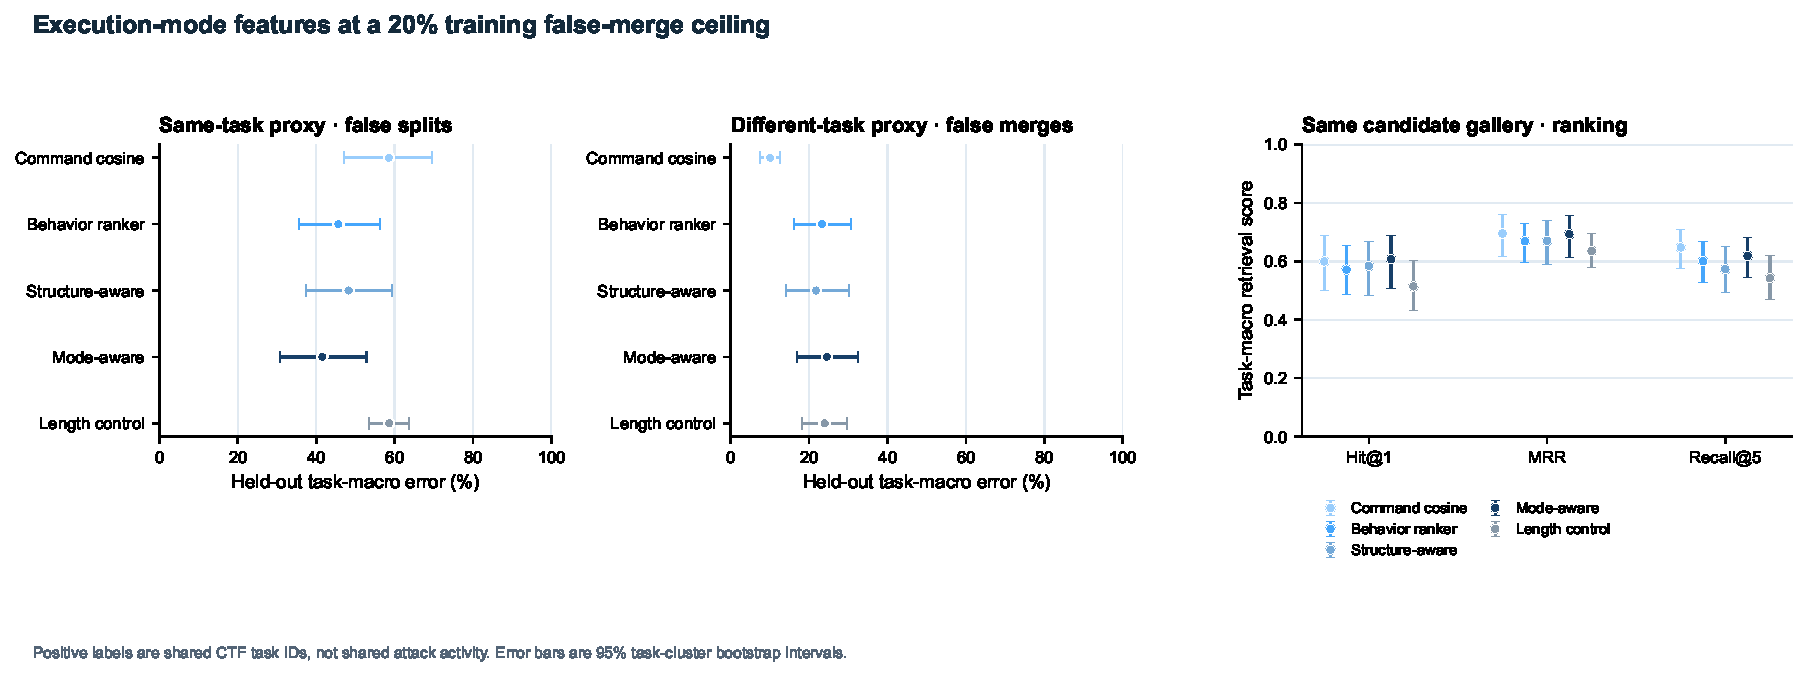
\includegraphics[width=\linewidth]{association_operating_points_v1.pdf}
\caption{Held-out challenge-matching errors and retrieval at the shared training-side 20\% false-merge target. Candidate galleries are identical across methods.}
\label{fig:operating-points}
\end{figure}

% Generated by scripts/plot_association_cases.py from audited JSON.
\subsection{Audited examples of changed decisions}

In the held-out CyBench challenge \texttt{back\_to\_the\_past}, a Human trace with 48 extracted commands and an Agent trace with 47 commands share the task label but have command-cosine similarity 0.215. The behavior ranker rejects the pair ($0.5088 < 0.5131$); the mode-aware ranker accepts it ($0.5482 \geq 0.5127$). The mode detector's raw Agent scores are 0.3683 and 0.7221, respectively. This pair illustrates how predicted mode information can change a borderline matching decision.

The same representation also introduces a cross-challenge link: a Human \texttt{back\_to\_the\_past} trace and an Agent \texttt{glacier-exchange} trace change from rejection ($0.4738 < 0.5131$) to acceptance ($0.5161 \geq 0.5127$). Figure~\ref{fig:association-cases} locates both the value and the design challenge: execution-mode context can recover cross-mode matches, while distinguishing the underlying task remains essential to controlling spurious links. Case selection and full trace identifiers are documented in the appendix.

\begin{figure}[t]
\centering
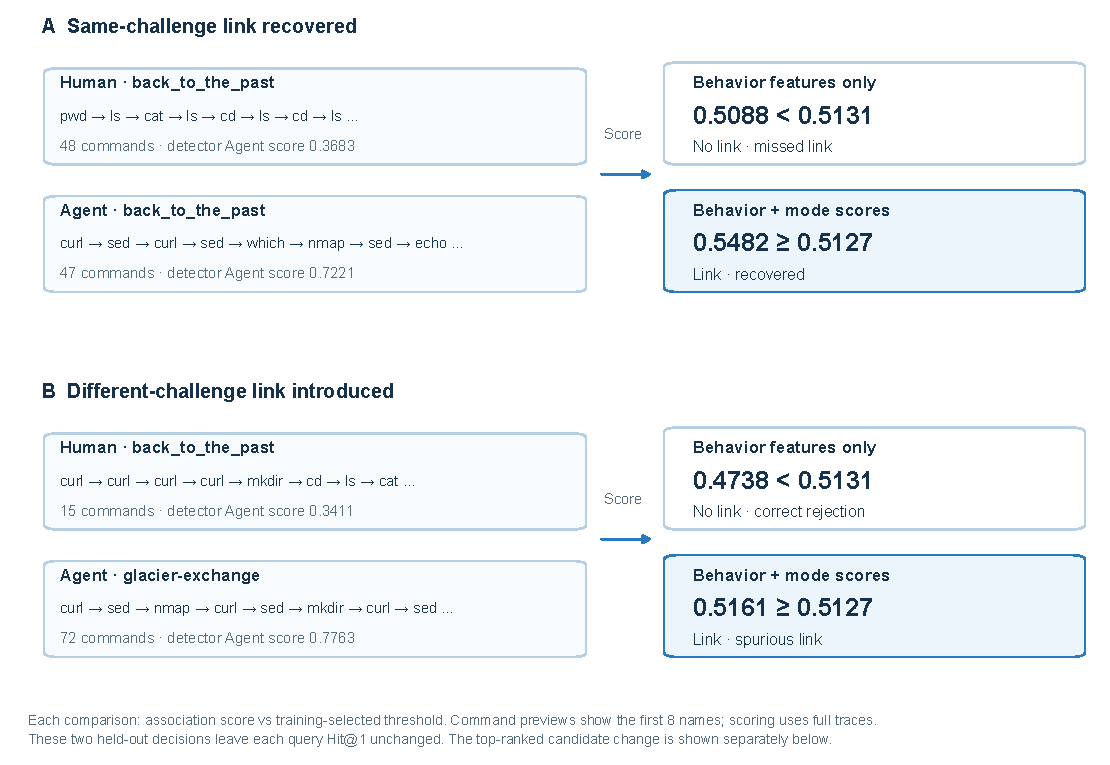
\includegraphics[width=\linewidth]{association_cases_v1.pdf}
\caption{Audited Human--Agent pairs from held-out CTF tasks. Each numeric comparison shows an association score against its training-selected threshold. The common 20\% training false-merge target permits method-specific thresholds. Only command-name previews are displayed; scoring uses complete normalized trajectories. Source labels are shown for interpretation, while the ranker uses predicted mode scores. These examples explain a recovered same-challenge link and a new cross-challenge error.}
\label{fig:association-cases}
\end{figure}

One held-out Human query gives a direct view of Hit@1. Its gallery contains 39 traces. The behavior-only ranker places a different-challenge Human trace first (score 0.6281) and the same-challenge Agent at rank 5. With predicted execution-mode scores, the Agent trace moves to rank 1 and the previous top result moves to rank 2; query Hit@1 changes from 0 to 1. This selected example illustrates the retrieval metric; the aggregate estimate uses every held-out query.

\begin{figure}[t]
\centering
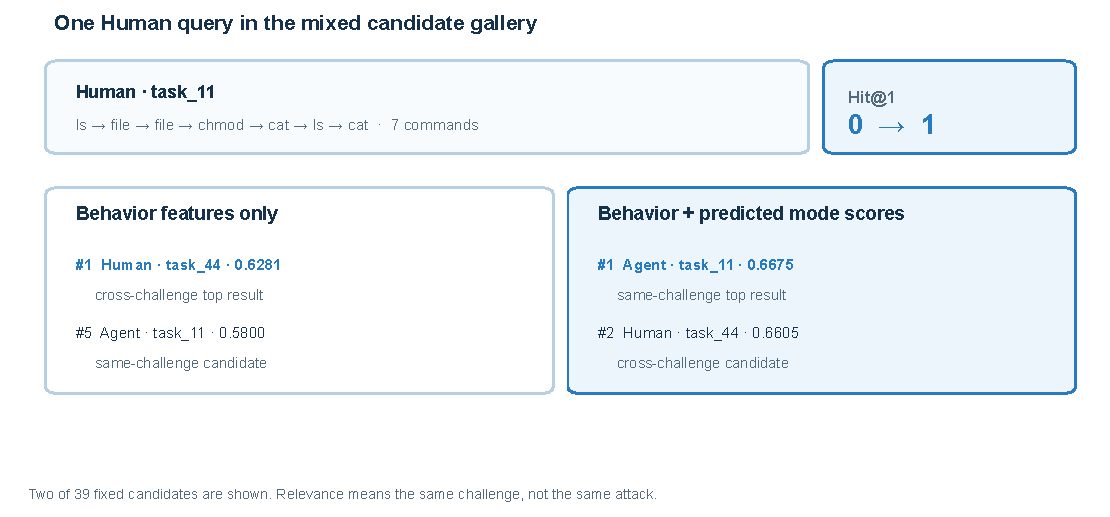
\includegraphics[width=\linewidth]{association_rank_case_v1.pdf}
\caption{A held-out Human query whose top-ranked candidate changes from a different-challenge Human trace to a same-challenge Agent trace after adding predicted execution-mode scores. Two candidates are shown from a fixed gallery of 39. Challenge relevance is an evaluation label, not an attack-activity label.}
\label{fig:association-ranking-case}
\end{figure}


\section{Conclusion}

Security investigations already use sequences, TTPs, and causal relations to associate activity evidence. These experiments show that execution-mode scores can shift this association profile: in CTF same-challenge retrieval, mode-aware ranking recovers more same-task Human--Agent pairs and also introduces more cross-task Human--Agent links. Command vocabulary supplies most of the measured classification signal; sequence statistics add no classifier-independent gain. The results support evaluating execution mode as an explicit association context. The next decisive evaluation requires human, scripted, and Agent executions under one sensor pipeline with independently labeled activities.

\appendix
\section{Full protocol and reproducibility}

\paragraph{Dataset composition.} The evaluated intersection contains 177 non-empty traces from 40 benchmark-qualified task groups. Human records are expert terminal inputs; Agent records are structured bash tool calls. Table~\ref{tab:appendix-data} gives the per-suite counts. The source is Cyber Task Horizons, pinned to revision \texttt{178c0da1800f9c07311e1b8d6c61dd8104e7b4ae} under CC BY 4.0. The task label denotes the same CTF challenge, not a shared intrusion or actor.

\begin{table}[t]
\centering
\caption{Composition of the evaluated public trace subset.}
\label{tab:appendix-data}
\small
\rowcolors{2}{PaleGray}{white}
\begin{tabularx}{0.84\linewidth}{>{\raggedright\arraybackslash}Xrrrr}
\toprule
\rowcolor{InkBlue}\textcolor{white}{Benchmark} & \textcolor{white}{Task groups} & \textcolor{white}{Human} & \textcolor{white}{Agent} & \textcolor{white}{Total} \\
\midrule
InterCode-CTF & 27 & 40 & 81 & 121 \\
CyBench & 6 & 8 & 18 & 26 \\
NYU CTF Bench & 7 & 9 & 21 & 30 \\
\rowcolor{PaleBlue}\textbf{Total} & \textbf{40} & \textbf{57} & \textbf{120} & \textbf{177} \\
\bottomrule
\end{tabularx}
\end{table}

\paragraph{Candidate construction.} Each non-empty trace in a held-out task group is a query. The gallery contains every other trace in the same benchmark and held-out fold, including both Human and Agent records. Query self-matches are removed by trace ID. A relevant candidate shares the benchmark-qualified task ID. Ties receive expected metric credit under a uniform random ordering. The random \Hit{} is the mean reciprocal gallery size at the query level, aggregated with equal benchmark weight.

\paragraph{Feature and training separation.} The input representation consists of normalized command names and coarse action labels derived by the pinned corpus parser. The association pair labels use only benchmark/task identity. The mode classifier trains on command TF--IDF unigram and bigram features. For training pairs, execution-mode features are generated by task-grouped inner cross-fitting; the outer held-out fold is not used to fit vocabulary, classification models, or the ranker. Candidate inclusion never depends on predicted or true mode.

\paragraph{Model specification.} Command and ordered-action representations use training-fold TF--IDF with sublinear term frequency. The execution-mode classifier is class-balanced logistic regression ($C=1$, maximum 3,000 iterations) over command-name unigrams and bigrams. Within each outer training fold, three task-grouped inner folds generate out-of-fold probabilities for the training traces; a classifier refit on the full outer training fold scores held-out traces. A Platt calibrator is fit to the training-task out-of-fold logits. Calibrated scores are used for the trace-label confusion matrix, classification, calibration, and selective-prediction diagnostics; association ranking uses the uncalibrated out-of-fold / held-out scores. The pair ranker is class-balanced logistic regression ($C=0.5$, maximum 3,000 iterations). Its behavior-only feature vector contains command cosine, ordered-action-bigram cosine, ProcGrep BPE/Jensen--Shannon similarity, and exponentially transformed log-command-count difference. The mode-aware variant adds the pair's predicted same-mode probability and absolute probability gap. For each training task group, up to 32 same-task pairs are sampled, alongside the same number of different-task pairs from the same benchmark; duplicate unordered pairs are removed. Both pair rankers use the same resulting pair set and labels.

\paragraph{Uncertainty.} Each reported interval resamples benchmark-qualified task groups within benchmark strata 5,000 times, preserving paired method comparisons and equal weighting of the three benchmarks. The intervals are conditional on each fixed task split and fitted model. Alternate seeds reuse the same traces and test split sensitivity; they are not independent samples or external replication.

\begin{table}[t]
\centering
\caption{Mode-aware minus task-supervised behavior \Hit{} change by task split.}
\label{tab:split-sensitivity}
\small
\rowcolors{2}{PaleGray}{white}
\begin{tabularx}{0.87\linewidth}{>{\raggedright\arraybackslash}Xrr}
\toprule
\rowcolor{InkBlue}\textcolor{white}{Split seed} & \textcolor{white}{Change} & \textcolor{white}{95\% task-cluster CI} \\
\midrule
20261030 (primary) & +0.0358 & [+0.0056, +0.0690] \\
20261130 & +0.0014 & [−0.0272, +0.0326] \\
20261230 & −0.0062 & [−0.0407, +0.0245] \\
20261330 & −0.0074 & [−0.0425, +0.0226] \\
20261430 & −0.0079 & [−0.0601, +0.0452] \\
20261530 & −0.0160 & [−0.0437, +0.0056] \\
\rowcolor{PaleBlue}\textbf{Alternate-split mean} & \textbf{−0.0072} & \textbf{[−0.0264, +0.0115]} \\
\bottomrule
\end{tabularx}
\end{table}

\begin{figure}[t]
\centering
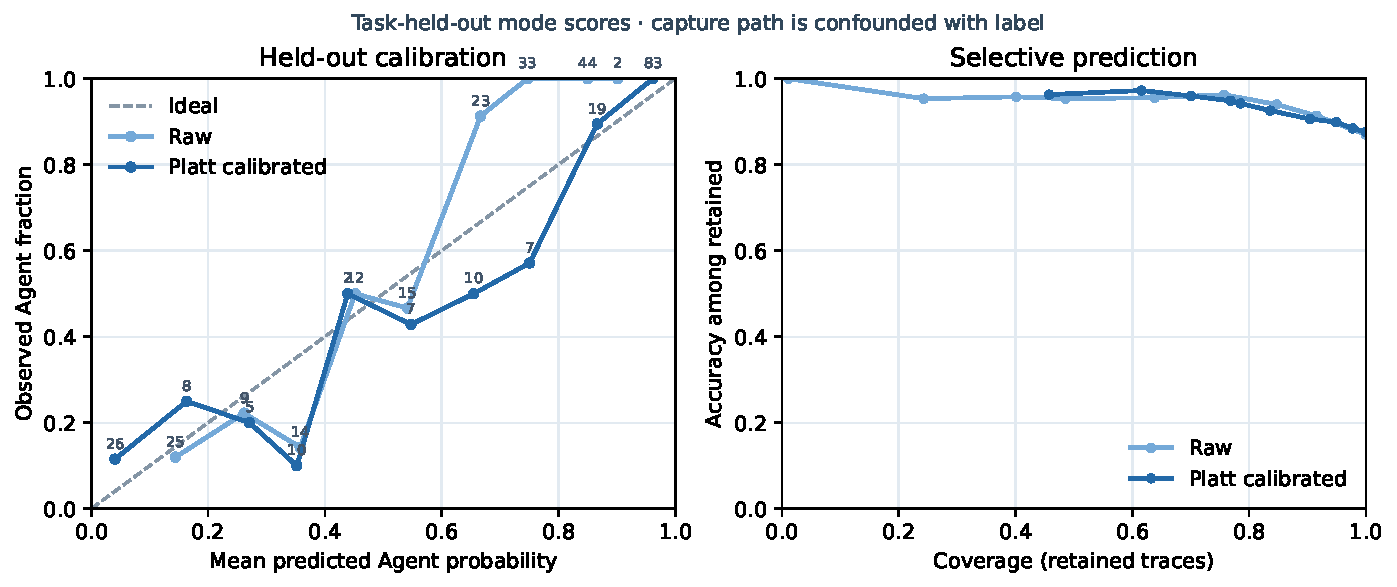
\includegraphics[width=\linewidth]{mixed_gallery_calibration.pdf}
\caption{Out-of-fold calibration and selective-prediction diagnostics. Scores describe Human/Agent record labels in the source release; capture path is confounded with the label.}
\label{fig:calibration}
\end{figure}

\paragraph{Pairwise error protocol.} The association-error experiment uses the same 177 traces and three benchmark-stratified outer task folds as the mixed-gallery study. Within each outer training partition, a second three-fold task-grouped cross-fit generates out-of-fold association scores for threshold selection. For each method, the threshold maximizes task-macro balanced accuracy over 101 empirical score quantiles and the observed score bounds; ties select the higher threshold. The outer test fold is scored once with the outer-training model and this fixed threshold. Pair features and pair-training labels are unchanged from the mixed-gallery rankers: benchmark/task identity constructs training positives and negatives, while the evaluator alone uses held-out task IDs.

For a query trace $q$, the false-split rate is the fraction of same-challenge candidates rejected, and the false-merge rate is the fraction of different-challenge candidates accepted. Candidate rates are averaged within each query, queries within each task, tasks within each benchmark, and benchmarks with equal weight. Task-macro balanced accuracy is $1 - (\mathrm{FNR}+\mathrm{FPR})/2$, where FNR and FPR denote these aggregated false-split and false-merge rates. The H--H, H--A, and A--A rates use the same query/task aggregation restricted to the indicated pair type. Pair rows are directed for query-level scoring; uncertainty resamples task groups, not pair rows.

The 95\% intervals use 5,000 paired task-cluster bootstrap samples within benchmark. Bootstrap draws condition on the fitted outer-fold models and the training-selected thresholds; they do not capture variability from repeating the complete nested fit. Pair-level outputs retain trace IDs, challenge-relevance labels, scores, and decisions; the worked-example JSON additionally includes allowlisted command names, but no raw logs, arguments, paths, or outputs. The reproducible implementation and figure code are in \texttt{scripts/run\_association\_error\_analysis.py}; the runnable notebook is \texttt{notebooks/08\_association\_error\_analysis.ipynb}.

\paragraph{Data source and license.} Cyber Task Horizons is pinned to commit \texttt{178c0da1800f9c07311e1b8d6c61dd8104e7b4ae} under CC BY 4.0. The manifest records selected source files, hashes, suite and task IDs, collection labels, and latest-attempt deduplication. Raw traces are fetched locally and are not redistributed by this repository. Task identity labels same-challenge retrieval relevance; shared intrusions are not annotated.

\paragraph{Reproduction.} From the repository root, install the locked CPU dependencies, download the pinned public traces, then run:

\begin{verbatim}
.venv/bin/python scripts/run_mixed_gallery.py --bootstraps 5000
.venv/bin/python scripts/run_association_error_analysis.py --bootstraps 5000 --threshold-grid 101
.venv/bin/python -m unittest discover -s tests -v
\end{verbatim}

The mixed-gallery run writes \texttt{results/mixed\_gallery.json}, task/query CSVs, held-out mode predictions, and three PDF/PNG figures. The association-error run writes \texttt{results/association\_error\_analysis.json}, pair-score, task-metric, and threshold CSVs, plus a PDF/PNG error-profile figure. Both result JSON files record the data revision, protocol version, evaluation definition, bootstrap method, and source hash. Figure-generation code remains in the corresponding experiment scripts.

\section{Follow-up feature and association protocol}

\paragraph{Feature ablation.} Four fixed inputs are compared: F0, log command count plus action proportions; F1, command-name TF--IDF unigrams and bigrams; F2, sequence transition, repetition, uniqueness, run-length, and short-trace statistics without command count; and F3, F1 concatenated with F2. Balanced logistic regression ($C=1$) and ExtraTrees (300 trees, depth 8, minimum leaf 3) are evaluated on six three-fold task-grouped splits. Vectorizers and models are fit only on training tasks. Estimates average each task across the six split seeds before a 5,000-draw benchmark-stratified task bootstrap. Repeated seeds are split-sensitivity checks, not independent replications.

\paragraph{Observation and order controls.} Prefix comparisons use matched task cohorts: 175 traces in 40 tasks for the two-command comparison, and 99 traces in 25 tasks for the four-command comparison. Full traces and prefixes are re-evaluated under the same task splits. On the four-command cohort, five fixed seeds shuffle aligned command/action events while preserving their counts. Paired intervals resample tasks within benchmark.

\paragraph{Model-source transfer.} Claude Opus, Claude Sonnet, and GPT-5.5 are each held out in turn. Tasks are also held out from training; test sets pair the held-out model's Agent traces with same-task Human records. Human test records recur across the three model panels, so the panels are dependent. This diagnoses model-source transfer on the current corpus rather than external validation.

\paragraph{Fixed-operating-point association.} The outer split uses three benchmark-stratified task folds with seed \texttt{20261030}. Each threshold is selected from inner task-held-out training predictions to minimize false splits subject to a task-macro false-merge ceiling of 10\%, 20\%, or 30\%. The 20\% ceiling is primary. Five methods share the same held-out candidates: command cosine, a behavior ranker containing command, action-bigram, ProcGrep, and length similarities, the behavior ranker plus fixed sequence statistics, the behavior ranker plus out-of-fold mode-agreement features, and a length-only control. Candidate inclusion is not conditioned on mode. Test false-merge rates are reported as observed and may differ from the training ceiling. Relevance is defined by the same CTF challenge. Results use 5,000 paired task-cluster bootstrap draws conditional on the fitted outer folds.

\paragraph{Audited worked examples.} Threshold examples C1--C3 are selected as the lexicographically first Human-query/Agent-candidate pairs in the recovered-link, introduced-link, and persistent-miss categories. Ranking example C4--C5 is selected from two held-out Human queries meeting a fixed criterion: behavior-only Hit@1 is zero, mode-aware Hit@1 is one, and at least one same-challenge Agent is tied at the top. In the selected InterCode-CTF query (trace \texttt{d209c425ee9ce2bf}; 39 candidates), behavior-only ranking puts the different-challenge Human trace \texttt{4cdc4644c4f559d9} first (score 0.6281) and the relevant Agent trace \texttt{1d9f0d5a2f0a520d} fifth (0.5800). Mode-aware ranking places the Agent first (0.6675) and the Human second (0.6605), changing query Hit@1 from 0 to 1. These are deliberately selected explanatory examples, not prevalence estimates. The extraction script independently refits the selected outer folds and verifies all frozen pair scores; the maximum absolute discrepancy is 0.0 and no task overlaps train and test. Full IDs, safe command-name previews, thresholds, scores, and ranks are in \texttt{results/association\_cases\_v1.json}. Figures are generated by \texttt{scripts/plot\_association\_cases.py}.

\paragraph{Reproduction.} With the pinned traces in the ignored \texttt{data/} directory, run:

\begin{verbatim}
.venv/bin/python scripts/run_feature_ablation.py
.venv/bin/python scripts/summarize_feature_contrasts.py
.venv/bin/python scripts/run_agent_model_transfer.py --bootstraps 5000
.venv/bin/python scripts/run_association_operating_points.py --bootstraps 5000 --threshold-grid 101
.venv/bin/python scripts/extract_association_cases.py --refit
.venv/bin/python scripts/plot_association_cases.py
.venv/bin/python scripts/plot_feature_ablation.py
.venv/bin/python scripts/plot_association_operating_points.py
\end{verbatim}

The feature and association notebooks are \texttt{notebooks/09\_feature\_ablation\_v1.ipynb} and \texttt{notebooks/10\_association\_operating\_points\_v1.ipynb}. Derived tables, predictions, thresholds, task-level scores, and figure-generation code are retained in \texttt{results/} and \texttt{scripts/}.

\begin{thebibliography}{99}
\bibitem{holmes} S. M. Milajerdi, R. Gjomemo, B. Eshete, R. Sekar, and V. N. Venkatakrishnan, ``HOLMES: Real-Time APT Detection through Correlation of Suspicious Information Flows,'' in \emph{2019 IEEE Symposium on Security and Privacy}, pp. 1137--1152, 2019. \href{https://doi.org/10.1109/SP.2019.00026}{doi:10.1109/SP.2019.00026}.
\bibitem{ostinato} S. K. Ghosh, K. Satvat, R. Gjomemo, and V. N. Venkatakrishnan, ``Ostinato: Cross-host Attack Correlation through Attack Activity Similarity Detection,'' in \emph{18th International Conference on Information Systems Security}, 2022. \href{https://arxiv.org/abs/2312.09321}{arXiv:2312.09321}.
\bibitem{poirot} S. M. Milajerdi, B. Eshete, R. Gjomemo, and V. N. Venkatakrishnan, ``POIROT: Aligning Attack Behavior with Kernel Audit Records for Cyber Threat Hunting,'' in \emph{Proceedings of the 2019 ACM SIGSAC Conference on Computer and Communications Security}, pp. 1813--1830, 2019. \href{https://doi.org/10.1145/3319535.3363217}{doi:10.1145/3319535.3363217}.
\bibitem{hercule} K. Pei, Z. Gu, B. Saltaformaggio, S. Ma, F. Wang, Z. Zhang, L. Si, X. Zhang, and D. Xu, ``HERCULE: Attack Story Reconstruction via Community Discovery on Correlated Log Graph,'' in \emph{Proceedings of the 32nd Annual Conference on Computer Security Applications}, 2016. \href{https://doi.org/10.1145/2991079.2991122}{doi:10.1145/2991079.2991122}.
\bibitem{atlas} A. Alsaheel, Y. Nan, S. Ma, L. Yu, G. Walkup, Z. B. Celik, X. Zhang, and D. Xu, ``ATLAS: A Sequence-based Learning Approach for Attack Investigation,'' in \emph{30th USENIX Security Symposium}, 2021. \href{https://www.usenix.org/conference/usenixsecurity21/presentation/alsaheel}{USENIX Security 21}.
\bibitem{actminer} M. Ma et al., ``ActMiner: Applying Causality Tracking and Increment Aligning for Graph-based Cyber Threat Hunting,'' \emph{Knowledge-Based Systems}, vol. 327, 2025. \href{https://doi.org/10.1016/j.knosys.2025.114169}{doi:10.1016/j.knosys.2025.114169}.
\bibitem{falcon} J. Tang, Y. Gao, X. Li, J. Li, S. Yu, and B. Fang, ``FALCON: Adaptive Cross-Domain APT Attack Investigation with Federated Causal Learning,'' in \emph{Proceedings of the Forty-first Conference on Uncertainty in Artificial Intelligence}, vol. 286, pp. 4113--4131, 2025. \href{https://proceedings.mlr.press/v286/tang25a.html}{PMLR 286}.
\bibitem{anthropic} Anthropic Threat Intelligence, ``Disrupting the First Reported AI-Orchestrated Cyber Espionage Campaign,'' 2025. \href{https://www.anthropic.com/news/disrupting-AI-espionage}{Report}.
\bibitem{mitrec0062} MITRE ATT\&CK, ``Anthropic AI-orchestrated Campaign (C0062),'' 2025. \href{https://attack.mitre.org/campaigns/C0062/}{Campaign record}.
\bibitem{unit42} Unit 42, ``Introducing Unit 42's Attribution Framework,'' 2025. \href{https://unit42.paloaltonetworks.com/unit-42-attribution-framework/}{Framework}.
\bibitem{cth} Lyptus Research, ``Cyber Task Horizons: Public Cyber Task Traces,'' dataset release, CC BY 4.0. \href{https://github.com/lyptus-research/cyber-task-horizons-data}{Repository}.
\bibitem{ait} AIT Austrian Institute of Technology, AECID, ``LLM User Shell Simulation,'' public research repository, 2026. \href{https://github.com/ait-aecid/llm-user-shell-sim}{Repository}.
\end{thebibliography}
\end{document}
